%%%%%%%%%%%%%%%%%%%%%%%%
\chapter{The NinjaCrane Attack}
% The implementation covers some of the implementation details of your project.
% This is not intended to be a low level description of every line of code that you wrote but covers the implementation aspects of the projects.
% This section is usually 3-5 pages.
%%%%%%%%%%%%%%%%%%%%%%%%
\label{chapter:ninja-crane-atk}

\section{Entry Points}

The implementation choice of the entry point infecting the workstation has been to create two equivalent entry points — the USB Ninja cable and the malicious mouse. Payloads stored on the USB Ninja cable can be triggered over BLE which makes it more interactive for a live demonstrator. The drawback of the USB Ninja cable is the storage capacity, too small to store the \emph{NinjaCrane} malware. The \emph{NinjaCrane} malware must be already downloaded or stored on the workstation (or on the device connected to this USB Ninja cable). To overcome this, a malicious mouse has been made. It offers a better flexibility as any board with USB-B connector can be placed and connected inside the mouse. This allows to store the malware directly inside the mouse.

\subsection{USB Ninja}

The BLE communication protocol used by the USB Ninja cable has been reverse-engineered by the Embedded Lab Vienna for IoT \& Security~\cite{ninja-cable-reverse}. From this work, a script controlling the USB Ninja cable from the BLE of a windows computer has been made with the help of the \texttt{bleak} python package.

Given the USB Ninja cable's Bluetooth MAC address, the script connects to its associated BLE GATT server. To trigger the payloads stored on the USB Ninja cable, two BLE packets are sent consecutively. The first one writes at BLE handle $\texttt{0x36}$ the password. The second packet writes at BLE handle $\texttt{0x36}$ either \texttt{A=L$\backslash$r$\backslash$n} or \texttt{B=L$\backslash$r$\backslash$n} to trigger the first or the second payload respectively. The script is used by the attacker's GUI; button \texttt{Deploy Payload} sends \texttt{A=L$\backslash$r$\backslash$n} and button \texttt{Trigger Attack A} sends \texttt{B=L$\backslash$r$\backslash$n} to the USB Ninja cable.

\subsection{Malicious Mouse}

The clean mouse is a Logitech M90 USB wired mouse. A DIY Tiny USB Hub~\cite{usb-diy-hub}, placed inside this mouse, splits the USB wired connection in order to connect both the mouse and a micro USB type-B male connector. A pre-programmed Adafruit Trinket M0 is plugged to this connector. The Trinket M0 is a HID-capable device that can emulate a keyboard or a mouse. Picture of this assembly can be found in~\autoref{fig:infected-mouse-photo}. The Trinket M0 is programmed using \href{https://circuitpython.org/}{\texttt{CircuitPython v8.2.0}} by placing in its associated USB drive two different files (\texttt{code.py} and \texttt{boot.py}). When the Trinket is plugged-in the \texttt{boot.py} and the \texttt{code.py} scripts are respectively executed. The first script will deactivate Midi, REPL and USB drive (but not HID). The second script executes the HID payload and then activates the USB drive where the malware is stored. 

\subsection{Payloads of the HID-capable Device}

The payload of the cable executes the following instructions: open Run command, open a hidden powershell terminal, write and execute a script that will detect internet connection, download a malware and execute it in background. Moreover, for a background persistence, a malware's shortcut is placed in the engineering workstation startup folder.

The payload of the mouse executes similar instructions: open Run command, open a hidden powershell terminal, and execute the malware in background. No internet connection is required as the malware is stored in the malicious mouse.


\section{Attacker's GUI}

No attacker's GUI are available to control the malicious mouse as the Trinket M0 has no wireless communication. But if the entry point is the USB Ninja cable, a python interface to control the attack can be used. This interface is shown in~\autoref{fig:gui}. Python interface has been written with \emph{PySimpleGUI} package in order to better illustrate the steps taken by adversary and simplify the attack explanations. This GUI is made of one interface modeling the attack progress on the ICS architecture and two buttons. The first button \texttt{Deploy Payload} will trigger the first payload stored on the USB Ninja cable. The second button \texttt{Trigger Attack A} will trigger the second payload stored on the USB cable.

\section{The \emph{NinjaCrane} Malware}

The \emph{NinjaCrane} malware is a python script that is converted into an executable file named \texttt{malwar3.exe}.

\subsection{MITM Script}

The MITM script is a .pyw extension python file for better flexibility and stealthiness. This script first by-pass the UAC consent prompt to execute itself with admin rights. It then waits for a trigger to perform the MITM attack on the polar crane.

\subsubsection{UAC Consent Prompt By-Passing}

First, the script detects if it runs with administrative privilege. If not it will exploit the \texttt{fodhelper.exe} weakness (i.e., \texttt{fodhelper.exe} elevates itself to run in a higher integrity level) to execute again itself with admin privilege. Otherwise it continues with the attack. 

To exploit the \texttt{fodhelper.exe} weakness, two register keys are created at \texttt{HKEY\_CURRENT\_USER$\backslash$Software$\backslash$Classes$\backslash$ms-settings$\backslash$shell$\backslash$open$\backslash$command}. The first key (\texttt{DelegateExecute}) is set to empty string and the second key (Nil) is set to the command to execute with higher integrity context (i.e., executes this python script again) as shown in~\autoref{fig:reg-uas-bypass}. No privilege are needed to modify and create those \texttt{HKEY\_CURRENT\_USER} register keys. Finally, the python script executes \texttt{C:$\backslash$$\backslash$Windows$\backslash$$\backslash$System32$\backslash$$\backslash$fodhelper.exe} to run itself again with higher privilege. 

\begin{figure}[H]
    \centering
    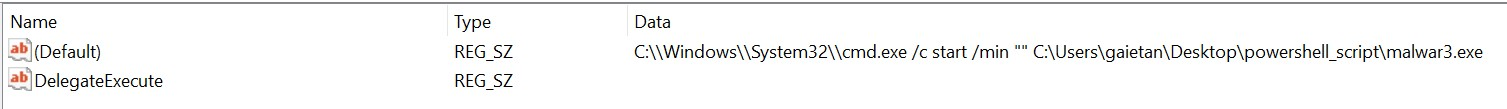
\includegraphics[width=\linewidth]{figures/reg-uac-bypass.jpg}
    \caption{Register keys created to By-Pass Windows Consent Prompt UAC}
    \label{fig:reg-uas-bypass}
\end{figure}

\subsubsection{Waiting for Attack Trigger}

Once the script executes with admin privilege it makes use of the \texttt{pydivert} package to listen and modify the packets sent by the workstation to the PLC. The \texttt{pydivert} package is itself based on Windows Packet Divert (named \texttt{WinDivert}), a capture-and-divert package for Windows. 

The script captures only the UMAS packets (i.e. packets from/to the engineering workstation's $503$ TCP port). The script extracts the key information e.g., \texttt{server\_nonce}, \texttt{client\_nonce}, \texttt{salts} \& \texttt{hash}, Unity Pro version, project name, project folder etc. 

\subsubsection{Data Exfiltration}

As soon as the script extracts the project folder it will try to exfiltrate over internet the\texttt{.STU} program and a text file with project information. The text file with project information is stored in the \texttt{$\backslash$Desktop$\backslash$powershell\_script$\backslash$extracted\_info.txt}. The script thus uploads from the workstation the two files on a \href{transfer.sh}{\texttt{transfer.sh}} server and sends an SMTP email with the corresponding urls with the use of the \href{https://mailtrap.io/}{\texttt{mailtrap}} solution. The attacker from outside, receiving this email can then download those two files as shown in~\autoref{fig:mailtrap-exfiltrate-data}.

This data exfiltration allows the adversary to perform aside an analysis of the .STU program running on the PLC and to better weaponize the malware. Indeed, as soon as the adversary has access to the program, it has access to the memory addresses of every variables, their use and their type. This allows the adversary to craft a valid authenticated packet to modify or read any of those variables. 

\subsubsection{Send Malicious Authenticated Packet}

\label{subsec:malicious-sent-packets}

When the adversary triggers the attack (or when mouse is plugged-in), the USB Ninja (or malicious mouse respectively) will write to a text file. The script is continuously reading this text file. In case of file modification, the script will start to send malicious authenticated packets. For a better cyberattack illustration purpose the following malicious packets are sent:

\begin{itemize}
    \item \textbf{Packet 1}: Sends a request to initiate the variables monitoring.
    \item \textbf{Packet 2}: Sets the rotation speed of the polar crane's rotation to 34 \% of the maximum motor's speed. 
    \item \textbf{Packet 3 \& 4}: Activate the polar crane's rotation. First is a rising edge (i.e., sets the corresponding internal variable to 1) the other one is a falling edge (i.e., sets the corresponding internal variable to 0).
    \item \textbf{Packet 5}:  Sets the rotation speed of the polar crane's rotation to 63 \% of the maximum motor's speed. 
    \item \textbf{Packet 6 \& 7}: Activate the polar crane's rotation. Those packets are needed in order for the polar crane to apply the previously set rotation speed.
    \item \textbf{Packet 8 \& 9}: Deactivate rotation. First is a rising edge,  the other one is a falling edge.
    \item \textbf{Packet 10}: Stops the PLC.
\end{itemize}

To sum up, the above packets will make the polar crane rotate slowly first, then fast, then completely stop the polar crane and the PLC. This scenario could be improved to also show that the attacker can extract the value of the internal variables. To send the malicious packet the script completely modifies a sent \texttt{MONTOR\_PLC} (i.e., \texttt{0x50}) packet with the corresponding Modbus data. \texttt{PyDivert} automatically recomputes the checksum. However the TCP sequence and acknowledgment numbers must be modified according to the modified packet length. This modification must apply to any fresh packet sent or received (i.e., the script synchronizes the ack and seq numbers in order to avoid duplicate ack/seq, TCP re-transmission, and connection loss).

\subsection{Converting a Python Script to an Executable \emph{Malwar3.exe}}

As the engineering workstation has no python environment the script must be compiled. To compile the python script in one file, the \texttt{pyinstaller} package (or its Graphical Interface equivalent, \texttt{auto-py-to-exe 2.36.0}) has been used. Moreover the Ultimate Packer for eXecutables (UPX) reduces the compiled binary's size. The executed command to compile the python script is: \texttt{pyinstaller --noconfirm --onefile --windowed --upx-dir "path/to/upx\_filr"  "path/to/malware\_script.pyw"}